%\documentclass[handout]{beamer}
\documentclass[ignorenonframetext]{beamer}
\usepackage{textpos}
\usepackage{graphicx}
\usepackage{pgf}
\usepackage{caption}
\usepackage{listings}
\usepackage{multimedia}
\usepackage{gensymb}
\usepackage{amsmath, mathrsfs}

\graphicspath{ {../tart_overview}{./fig} }

% \captionsetup[figure]{labelformat=empty}% redefines the caption setup of the figures environment in the beamer class.

\usetheme{Boadilla}
\usefonttheme{serif}
% \mode<presentation>
% {
%  \usefonttheme{serif}
% % \useoutertheme{sidebar}
% %   \logo{\includegraphics[height=1cm]{elec_logo.pdf}}
% }

\title[TART]{An Overview of the\\Transient Array Radio Telescope}
\author[Molteno]{Tim Molteno}

\institute[Otago]
{
  Electronics Research Foundation (New Zealand) \\
  \& \\
  Department of Physics,
  University of Otago (New Zealand) \\
  \& \\
  Department of Physics \& Electronics,
  Rhodes University (South Africa) \\
  \vspace{2cm}
  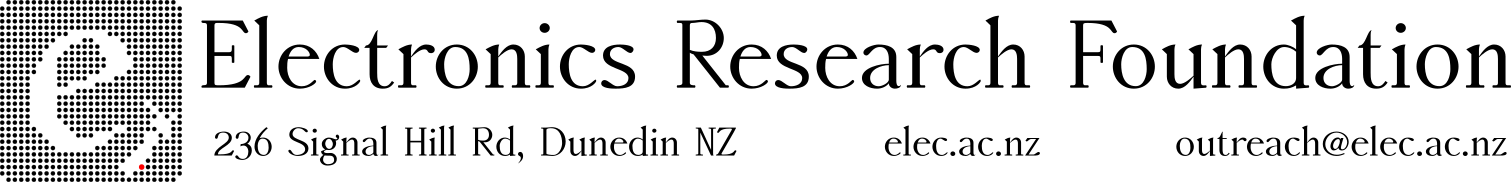
\includegraphics[width=0.6\linewidth]{../tart_overview/fig/elec_header_font.pdf}
}

\logo{\pgfputat{\pgfxy(-0.72,7.7)}{\pgfbox[center,base]{\includegraphics[width=1cm]{../tart_overview/fig/elec_logo.pdf}}}}

\date[IUB Nov 2025] % (optional, should be abbreviation of conference name)
{}

\begin{document}


% Abstract: In this talk I'll give an overview of Africa's newest radio telescope, the TART, recently installed in Mauritius in a joint effort between SARAO, the University of Otago (NZ). I'll talk about TARTs origins, it's design and open-source philosophy as well as the upcoming project to install TART telescopes in the SKA African partner nations. I'll also include some details about improvements that will appear in TART-3, the next version of TART!

\begin{frame}
  \titlepage
\end{frame}



\mode<all>
{
\usebackgroundtemplate{\includegraphics[height=\paperheight]{fig/meerkat.jpg}}
\begin{frame}[plain]
\end{frame}
}
\mode<all>{\usebackgroundtemplate{}}

\mode<all>
{
\usebackgroundtemplate{\includegraphics[height=\paperheight]{fig/MeerKAT_GalacticCentre_image.jpeg}}
\begin{frame}[plain]
\end{frame}
}
\mode<all>{\usebackgroundtemplate{}}

% \begin{frame}{MeerKAT: The Centre of our Galaxy}
%  \begin{center}
%   \includegraphics[width=\linewidth]{fig/MeerKAT_GalacticCentre_image.jpeg}
%  \end{center}
%
% \end{frame}


\mode<all>
{
\usebackgroundtemplate{\includegraphics[height=\paperheight]{fig/ghana.jpg}}
\begin{frame}[plain]
\end{frame}
}
\mode<all>{\usebackgroundtemplate{}}


% \begin{frame}{Abstract}
%  I will introduce the Transient Array Radio Telescope. Developed here in the Department of Physics at Otago University, this is the worlds smallest (and cheapest) aperture synthesis radio telescope -- that is a telescope that creates images of the radio sky. It is now being used by astronomers working on the Square Kilometer Array, the worlds largest radio telescope -- as an instrument that can be used to both develop new algorithms for radio astronomy and also to teach students about how radio telescopes work. I will describe the instrument and how it works, as well as giving an overview of the upcoming projects involving this telescope in Africa.
% \end{frame}

% \begin{frame}
%   \tableofcontents
%   % You might wish to add the option [pausesections]
% \end{frame}

\section{Origins}

\begin{frame}
\begin{columns}[T]
 \begin{column}{0.48\linewidth}
  \includegraphics[width=\linewidth]{fig/meerkat_ground_view.jpg}
\begin{block}{SKA, MeerKAT, VLA \ldots}
\begin{itemize}
\item Incredibly sensitive
\item Narrow field of view
\item Total cost: huge
\item Distant Universe
\end{itemize}\end{block}
 \end{column}
% % Column 2 (vertical line)
%     \begin{column}{.02\textwidth}
%         \rule{.1mm}{0.7\textheight}
%     \end{column}

\begin{column}{0.48\linewidth}
  \includegraphics[width=\linewidth]{fig/zambia_array.jpg}
\begin{block}{TART}
\begin{itemize}
 \item Lower sensitivity
 \item Massive field of view.
 \item Nearby Universe
 \item Cosmic Rays, Transients.
\end{itemize}

\end{block}
\end{column}
\end{columns}
\end{frame}%



%
% \begin{frame}
%    \includegraphics[width=\linewidth]{fig/zambia_array.jpg}
% \end{frame}
% \begin{frame}{Goals of the workshop}
% \begin{}
%
% \end{frame}
% \section{Origins of TART}

% \begin{frame}{TART: Evaluation}
%    \includegraphics[width=\linewidth]{fig/project_map_14.png}
% \end{frame}
%

%  \begin{columns}
%   \begin{column}{0.5\linewidth}
%   \begin{center}
%     
\includegraphics[height=0.4\textheight]{fig/antenna.jpg}
%   \end{center}
%   \end{column}
%   \begin{column}{0.5\linewidth}
%    
\includegraphics[width=\textwidth]{fig/antenna.jpg}
%   \end{column}
%  \end{columns}
% 

% \section{Aperture synthesis Radio Telescopes}

% 
% \begin{center}
%   \includegraphics[width=0.45\linewidth]{fig/RadioNightSky_med.jpg}
%   \includegraphics[width=0.45\linewidth]{fig/green_bank.jpg}
% \end{center}
% \end{frame}

% \begin{frame}{Aperture synthesis Radio Telescopes}
% \begin{center}
%   \includegraphics[width=\linewidth]{fig/vla_large.jpg}
% \end{center}
% \end{frame}


% \begin{frame}{MeerKAT: Africa is a world-leader in radio astronomy}
% \begin{center}
%   \includegraphics[width=\linewidth]{fig/2018-MeerKAT-5-1030x355.jpg}
% \end{center}
% \begin{itemize}
%  \item 13.5 meter antennas. 143 $m^2$
%  \item 64 of them!
%  \item Frequency Range: 900 MHz - 1670 MHz
%  \item SKA pathfinder
% \end{itemize}
%
% \end{frame}


% \begin{frame}{MeerKAT: The Centre of our Galaxy}
%  \begin{center}
%   \includegraphics[width=\linewidth]{fig/MeerKAT_GalacticCentre_image.jpeg}
%  \end{center}
%
% \end{frame}



\section{Instrument Design}

% \frame{\tableofcontents[currentsection]}

% 
% \begin{frame}
%   \includegraphics[width=\linewidth]{fig/rhodes_opening.jpg}
% \end{frame}
% 
% \begin{frame}
%   \includegraphics[width=\linewidth]{fig/rhodes_photo_array.jpg}
%   \includegraphics[height=0.4\textheight]{fig/rhodes_photo_elec.jpg}
% \end{frame}



% \begin{frame}{TART: Overview}
%    \includegraphics[width=\textwidth]{fig/drone_view_rhodes.jpg}
%    \centering{all-sky  $\cdot$ 24 antennas $\cdot$ real-time $\cdot$ open-source $\cdot$ imaging interferometer }
% \end{frame}




% \mode<all>
% {
% \usebackgroundtemplate{\includegraphics[height=\paperheight]{fig/tart_udm_array.jpg}}
% \begin{frame}[plain]
% \end{frame}
% }
% \mode<all>{\usebackgroundtemplate{}}


\begin{frame}{Real-time, all-sky radio telescope}
 \includegraphics[width=\textwidth]{fig/browser_view.png}
\end{frame}

\begin{frame}
\begin{center}
\includegraphics[width=0.8\linewidth]{fig/spotless-mu-udm.png}
 \end{center}
\end{frame}

\subsection*{Open Source}


% \begin{frame}{TART-2: Installation in South Africa}
% \begin{center}
%   \includegraphics[width=0.9\linewidth]{fig/rhodes_photo_array.jpg}
% \end{center}
% \begin{itemize}
%  \item 0.025 meter antennas. 0.0005 $m^2$.
%  \item Frequency Range: 1575.42 MHz ($\pm 4$)
%  \item Dunedin, NZ, Rhodes \& Stellenbosch South Africa.
% \end{itemize}
% \end{frame}
% 
% \begin{frame}
% \vspace{1cm}
%   \includegraphics[width=\linewidth]{fig/rhodes_news_sa.jpg}
% \end{frame}

\begin{frame}{Open-source design}
  \centering\url{https://github.com/tart-telescope}
 \begin{columns}
  \begin{column}{0.4\linewidth}
    \begin{itemize}
      \item Designed for Research
      \item Github: Hardware
      \item Github: Software
      \item Github: Documentation
    \end{itemize}
    
    Contributors:
    \begin{itemize}
      \item Dunedin, NZ
      \item Rhodes, ZA
      \item Stellenbosch, ZA
      \item SARAO, ZA
      \item EMSS Antennas, ZA
      \item IUB (Bangladesh)
    \end{itemize}
  \end{column}
  \begin{column}{0.6\linewidth}
    \includegraphics[width=\linewidth]{fig/screenshot_github.png}
  \end{column}
  \end{columns}
\end{frame}

 

\mode<all>
{
\usebackgroundtemplate{\includegraphics[height=\paperheight]{fig/TART_Bangladesh.jpg}}
\begin{frame}[plain]
\end{frame}
}
\mode<all>{\usebackgroundtemplate{}}


% \begin{frame}{TART Electronics}
%  \includegraphics[width=\textwidth]{fig/tart3_boxed.jpg}
% \end{frame}
%
% \begin{frame}{TART Features}
%  \begin{columns}
%   \begin{column}{0.4\linewidth}
%     \begin{itemize}
%     \item 24-Radio Receivers
%     \item Correlator works in real time!
%     \item Each radio: 2.5 MHz bandwidth
%     \item Real-time visibilities
%     \item Stored in the cloud
%     \end{itemize}
%   \end{column}
%   \begin{column}{0.6\linewidth}
%     \includegraphics[width=\linewidth]{fig/tart3.jpg}
%   \end{column}
% \end{columns}
% \pause
%     \begin{block}{Field of View}
% 20 thousand square degrees.
%     \end{block}
%     \begin{block}{New Developments}
% The hardware is constantly being developed.
%     \end{block}
% \end{frame}


% \begin{frame}[containsverbatim]
% \frametitle{TART API: Access data from anywhere}
% TART data and control are done throught a web-based API.
%
% \centering{\url{https://api.elec.ac.nz/tart/tart3-test/}}
%
% \begin{lstlisting}[language=Python, frame=single, basicstyle=\footnotesize]
%  import requests
%
%  api_endpoint = "https://api.elec.ac.nz/tart/tart3-test/api/"
%  r = requests.get(api_endpoint + "/v1/imaging/vis")
%  print(r.json())
% \end{lstlisting}
%
% \end{frame}

% \begin{frame}{Synthesis Imaging}
% Measure complex visibility $V_{ij}$ by correlating signals from antenna $i$ and $j$.
% \[ V_{ij} = \frac{1}{T} \int_0^T E_i(t) E_j^{\star}(t) dt \]
% \begin{columns}
%  \begin{column}{0.55\linewidth}
% \begin{enumerate}
%  \item 276 Pairs of antennas
%  \item 16.368 MHz sampling rate per antenna
%  \item Real-time correlation in FPGA
%  \item 4.5 Giga MAC per second
%  \item T $\sim$ 1 second
% \end{enumerate}
%  \end{column}
%  \begin{column}{0.45\linewidth}
%  \includegraphics[width=\linewidth]{fig/papilio_pro.jpg}
%  \end{column}
% \end{columns}
% 
% \end{frame}
% 
% \begin{frame}{Synthesis Continued...}
% Fourier transform relationship between radio sky brightness $I(l,m)$ and
% visibility $V(u,v)$,
% \[
%   V(u,v) = \int I(l,m) e^{2\pi j(lu  + mv)} dl dm
% \]
% Obtain $I(l,m)$ through inverse Fourier transform of $V(u,v)$, 
% \[
%  I(l,m) = \mathscr{F}^{-1}\{V(u,v)\}
% \]
% where $V(u,v)$ is the visibility function sampled in the $uv$-plane at the locations of each antenna $(u_{ij},v_{ij})$ pair. 
% \end{frame}
% 

% \section{Expected \& Unexpected Results}

% \begin{frame}{Tart Imaging Results}
% \begin{center}
% \includegraphics[width=0.6\linewidth]{fig/tart_snapshot.pdf}\\
%  \url{https://tart.elec.ac.nz/old/strange_flyby.webm}
%  \end{center}
% \end{frame}


% 
% 
% \begin{frame}{The Dirty Image}
% For the TART telescope there are 24 antennas, 
% and 522 antenna pairs
% \begin{columns}
%  \begin{column}{0.5\textwidth}
%  \begin{figure}
% \includegraphics[width=\linewidth]{../../papers/2019_iceaa/uv_plane_init.pdf}
% \caption{U-V antenna pairs}
%  \end{figure}
%  \end{column}
%  \begin{column}{0.5\textwidth}
%  \begin{figure}
%  \includegraphics[width=\linewidth]{fig/beam_2017_10_21_19_38_39_UTC.png}
% % \includegraphics[width=\linewidth]{/home/tim/github/projects/max/phd/talk/nzip/pdf/dirty_beam_power_init.pdf}  
% \caption{Inverse Fourier Transform}
%  \end{figure}
%  \end{column}
% \end{columns}
% 
% \end{frame}
% % 
% % 
% % \begin{frame}{Swithing it on: Uncalibrated Image}
% % \begin{figure}
% % \includegraphics[height=0.9\textheight]{../../papers/2019_iceaa/uncalibrated_image.png} 
% % \end{figure}
% % \end{frame}
% % 
% % 
% % % \begin{frame}{CLEAN: H\"ogbom 1974}
% % % \begin{columns}
% % %  \begin{column}{0.5\linewidth}
% % % %  \includegraphics[width=\linewidth]{2017_10_21_19_38_39_UTC_uvfits_difmap.png}
% % %   \end{column}
% % %  \begin{column}{0.5\linewidth}
% % %   Image is the sum of point sources and a residual
% % %   \begin{eqnarray*}
% % %  I(l,m) & = & A_0 \delta(l_0, m_0) + I_0(l,m) \\
% % %  I_0(l,m)  & = & A_1 \delta(l_1, m_1) + I_1(l,m) \\
% % % 	   & = & \ldots
% % %   \end{eqnarray*}
% % %  \end{column}
% % % \end{columns}
% % % \end{frame}
% % 
% % 
% 
% 
% \begin{frame}{Calibrated Clean Image}
% \begin{center}
% \includegraphics[height=0.9\textheight]{{../../papers/2019_iceaa/tart_clean.png}}
% \end{center}
% \end{frame}


\section{TART Workshops}

\mode<all>
{
\usebackgroundtemplate{\includegraphics[height=\paperheight]{TART_map_bd.png}}
\begin{frame}[plain]
\end{frame}
}
\mode<all>{\usebackgroundtemplate{}}

% \frame{\tableofcontents[currentsection]}

% \begin{frame}{Workshops: Building the TART Community}
%  \begin{columns}
%   \begin{column}{0.4\linewidth}
% 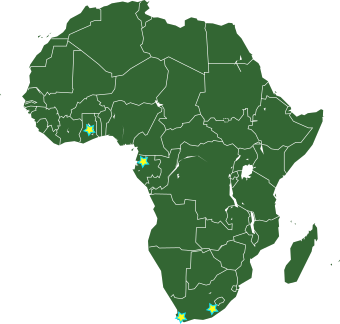
\includegraphics[width=\linewidth]{fig/Africa.pdf}
%   \end{column}
%   \begin{column}{0.6\linewidth}
%   \begin{itemize}
%    \item Week-long workshop
%    \item Mornings: Lectures on radio astronomy
%    \item Afternoons: Building a TART
%    \item Collaborations
%    \item Work with TART data
%   \end{itemize}
% \end{column}
%  \end{columns}
%  \centering
%    \includegraphics[width=0.71\linewidth]{fig/workshop-partners.png}
% \end{frame}
%


\end{document}
